\chapter{Theoretische Grundlage}
\label{sec:theorie}

% Dieser Abschnitt erklärt was Atmospärische Myonen sind
% und warum sie in der Myographie angewandt werden.
% Danach wird die Funktionsweise der Myographie erklärt,
% sowie deren Anwendungsbeispiele.

% solange nicht umstruturiert:
Dieser Abschnitt behandelt die theoretischen Grundlagen der Myographie.
Als Erstes werden atmosphärische Myonen vorgestellt, auf deren Absorption
die Myographie basiert. 

\section{Atmosphärische Myonen}

Myonen sind geladene Leptonen mit einer Ruhemasse von 
$m_{0} \approx \SI[]{106}[]{MeV}$ 
\cite{PDG2020}
und werden in der Atmosphäre aus der 
geladenen kosmischen Strahlung erzeugt (deshalb auch
kosmische Myonen genannt).
%  \marktodo{woraus besteht kosmische strahlung} 
Die kosmische Strahlung besteht im Allgemeinen aus hochenergetischen Teilchen,
welche von der Sonne, der Milchstraße oder fernen Galaxien kommt.
Die kosmische Strahlung ist beschreibbar über das Potenzgesetz   
\begin{equation*}
    \frac{\mathrm{d}N}{\mathrm{d}E}\thicksim E^{-\gamma}.
\end{equation*}
$N$ steht für die Anzahl an Teilchen und $E$ für die Energie.
$\gamma$ ist der sog. \textit{spektrale Index}. 
Für $E \leq 10^{15,5}\,\mathrm{eV}$ gilt $\gamma = \num{2,7}$ \cite{Gaisser16CR}. 

Die geladene kosmische Strahlung wechselwirkt mit den Stickstoff-, Sauerstoff- und 
Argonatomen in der Erdatmosphäre und erzeugt Luftschauer bestehend aus Hadronen, 
einem elektromagnetischen Teil, sowie Myonen.

Zur Produktion der Myonen wird zwischen den konventionellen 
und prompten Myonen unterschieden \cite{Gaisser16CR}.
Konventionelle Myonen entstehen aus Zerfällen von Pionen und Kaonen:
\begin{align*}
    \pi^{+} \to \mu^{+} + \nu_{\mu},\quad  & K^{+} \to \mu^{+} + \nu_{\mu}, \\
    \pi^{-} \to \mu^{-} + \overline{\nu_{\mu}},\quad  & K^{-} \to \mu^{-} + \overline{\nu_{\mu}}.
\end{align*}
Da $\pi$ und $K$ Mesonen eine verhältnismäßig lange Lebensdauer 
haben mit \\ 
$\tau_{\pi^{\pm}} = \SI[]{2.6033 \pm 0.0005 e-8}[]{s}$ und 
$\tau_{K^{\pm}}  = \SI[]{1.2380 \pm 0.0020 e-8}[]{s}$
und somit vor ihrem Zerfall 
mit der Atmosphäre wechselwirken und Energie verlieren,
besitzt das Energiespektrum jener Myonen den Spektralindex $\gamma=\num[]{3,7}$ \cite{Gaisser16CR}.

Prompte Myonen entstehen aus dem Zerfall von schwereren, meist charmhaltigen Hadronen wie z.B.:
\begin{align*}
    D^{0} &\to K^{-} + \mu^{+} + \nu_{\mu}, \\
    \varLambda _{c}^{+} &\to p + \mu^{+} + \mu^{- }.
\end{align*}
Da die Lebensdauer jener Hadronen jedoch sehr kurz ist,
$\tau_{D^{0}}  = \SI[]{410.1 \pm 1.5 e-15}[]{s}$ und 
$\tau_{\varLambda _{c}^{+}}  = \SI[]{202.4 \pm 3.1 e-15}[]{s}$,
zerfallen sie fast instantan, sodass sie ihre gesamte Ursprungsenergie an die entstehenden Teilchen
weitertragen können. Daher erben prompte Myonen den
Spektralindex $\gamma = \num[]{2,7}$ der geladenen kosmischen Strahlung.

Abb. \ref{fig:prompt_muonflux} zeigt, dass für $E_\mu < \SI[]{e4}[]{GeV}$
$> 99\%$ konventionelle Myonen sind . 
Prompten Myonen werden erst für $E_\mu > \SI[]{e5}[]{GeV}$
relevant und dominant ab $E_\mu > \SI[]{2 e6}[]{GeV}$

\begin{figure}[h]
    \centering
    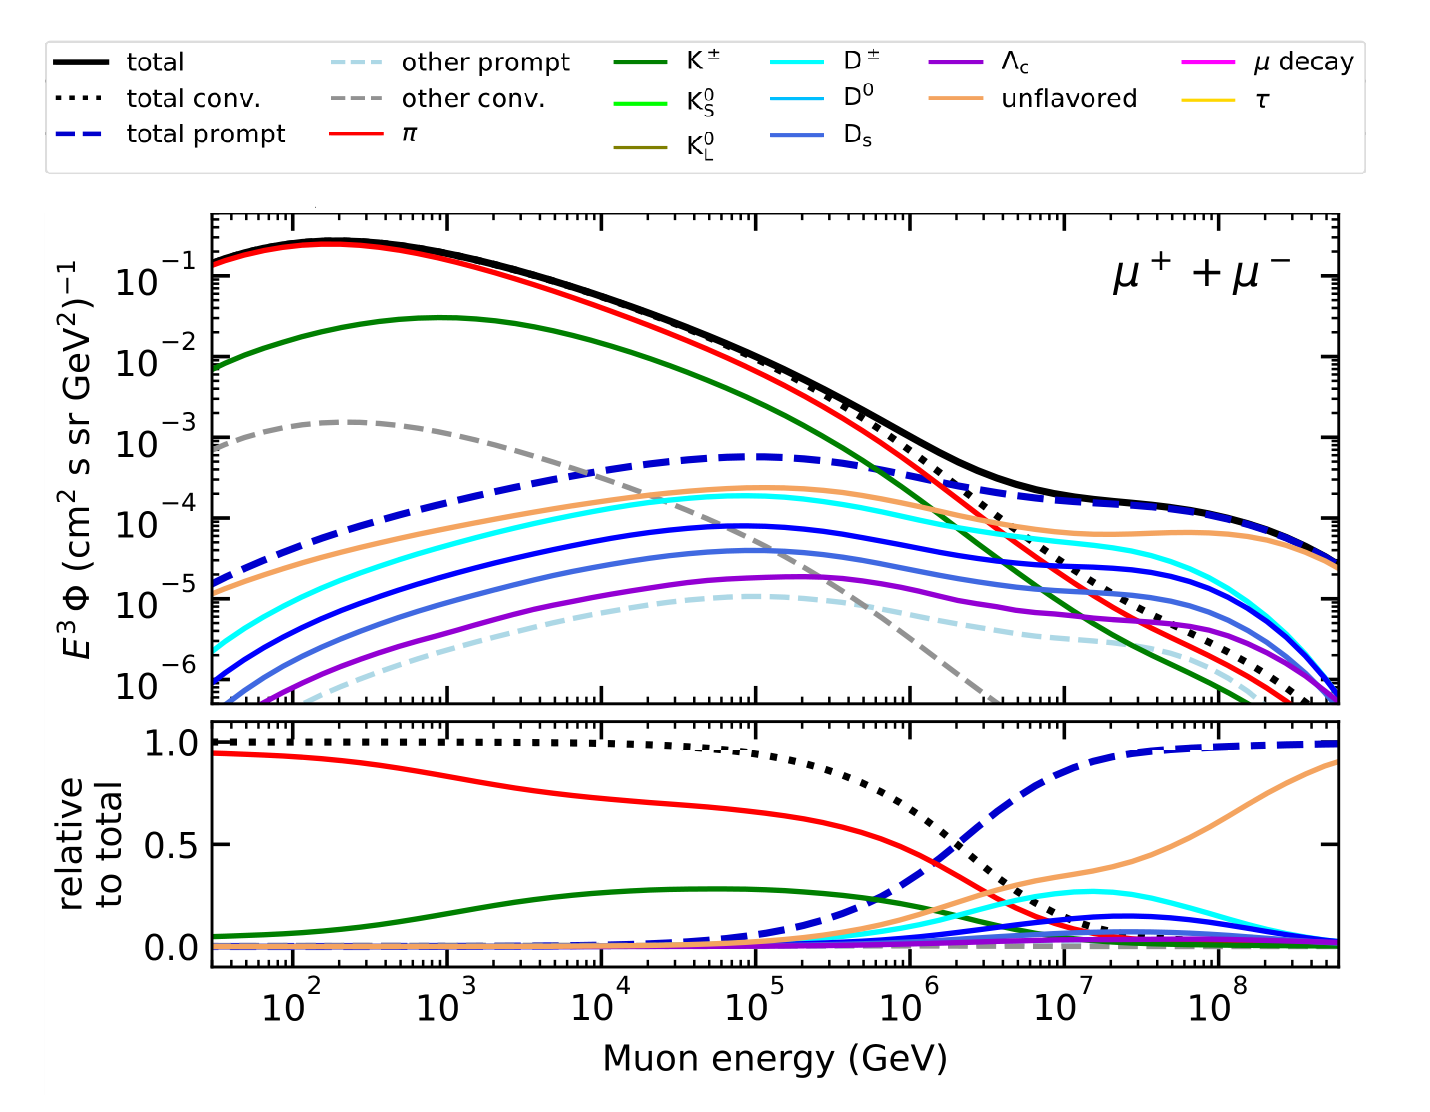
\includegraphics[width=0.8\textwidth]{muon_flux_fedynitch.png}
    \caption{Energiefluss atmosphärischer Myonen aufgeteilt nach den
     erzeugenden Hadronen, sowie deren relativen Beiträge,
      simuliert mit MCEq \cite{Fedynitch_2019}}
    \label{fig:prompt_muonflux}
\end{figure}

%%%%%%%%%%%%%%%%%%%%%%%%%%%%%%
% 2. Sektion plots und Reichweite
%%%%%%%%%%%%%%%%%%%%%%%%%%%%%%

% \newpage

% TODO heute
% 1: Warum Myonen:
%     - rel hohe Lebensdauer bei geringerer Wechselwirkungsrate 
%     -> hohe Reichweite

%     PLOT 
%     - Reichweite Plot aus Alexandrov

% 2: Myonen Spektrum

%   - Myonen auf sea level am häufigsten (alexandrov)
%     Zhang plot MYONEN RATE
    
%  todospäter 
%
% - wechselwirkungen (alexandrov)
%     - Wirkungsquerschnitt von röntgenstrahlung und Myonen vergleichen
% %
%   weiteres zu myonen spektrum: \\
%   
%   meiste myonen kommen aus vertikaler richtung

Auf Meereshöhe liegt die Flussdichte von Myonen typischerweise bei ca. 
$1 \; \frac{\mathrm{Myon}}{\mathrm{cm}^2 \; \mathrm{min}}$.  \cite{PDG2020} \cite{Schouten2019}

Da die Dichte des Erdreichs wesentlich höher ist als die der Atmosphäre,
nimmt die Myonenrate mit steigender Tiefe rapide ab,
wie in Abb. \ref{fig:Tiefenrate} zu sehen ist.

Die Reichweite kosmischer Myonen ist in Abb. \ref{fig:reichweite} zu sehen.

\begin{figure}[h]
    \centering
    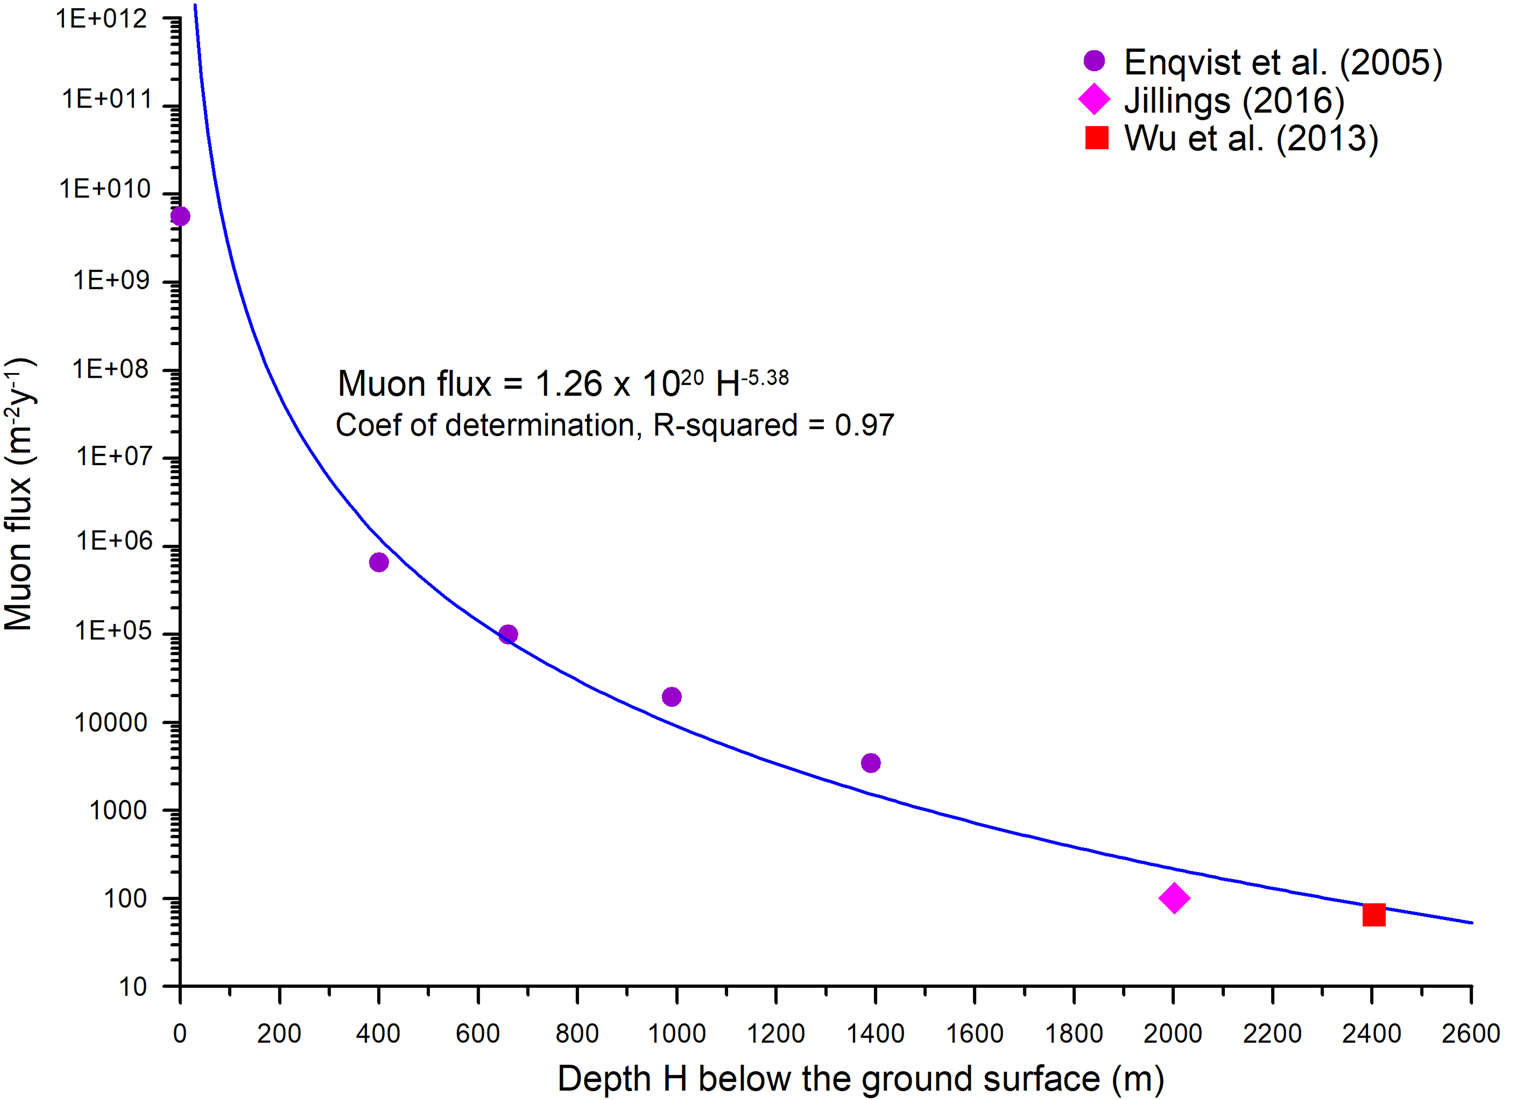
\includegraphics[width=0.7\textwidth]{Zhang_2020_muon_depth.png}
    \caption{
        Myonen Fluss gegen Tiefe unterhalb der Erdoberfläche.
        Mehrfarbig sind in verschiedenen Tiefen Messungen des Myonenflusses eingetragen.
        \cite{zhang2020}}
    \label{fig:Tiefenrate}
\end{figure}

\begin{figure}[h]
    \centering
    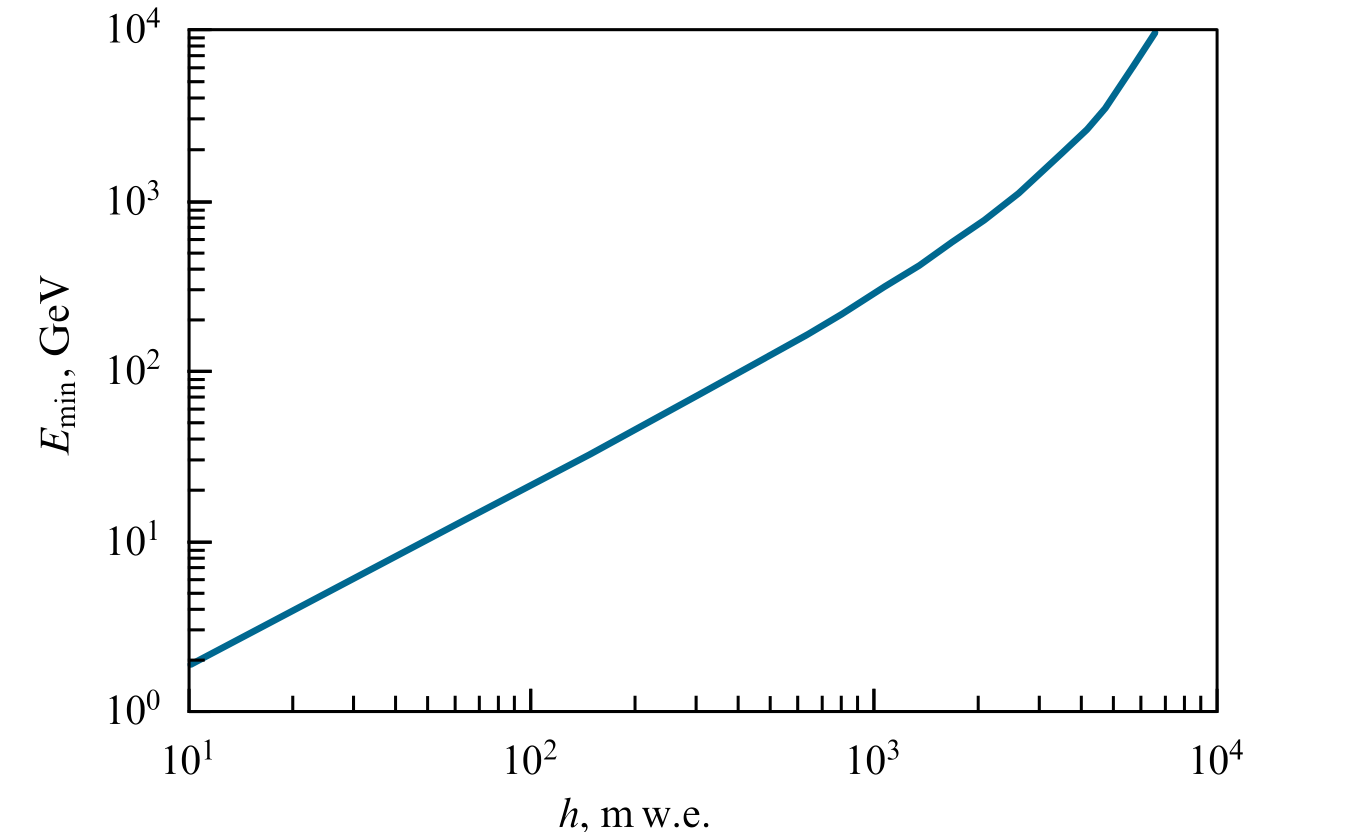
\includegraphics[width=0.7\textwidth]{reichweite.png}
    \caption{
        Die Reichweite von Myonen in $mwe$
        \cite{Alexandrov2017}}
    \label{fig:reichweite}
\end{figure}